\let\negmedspace\undefined
\let\negthickspace\undefined
\documentclass[journal]{IEEEtran}
\usepackage[a5paper, margin=10mm, onecolumn]{geometry}
%\usepackage{lmodern} % Ensure lmodern is loaded for pdflatex
\usepackage{tfrupee} % Include tfrupee package

\setlength{\headheight}{1cm} % Set the height of the header box
\setlength{\headsep}{0mm}     % Set the distance between the header box and the top of the text

\usepackage{gvv-book}
\usepackage{gvv}
\usepackage{cite}
\usepackage{amsmath,amssymb,amsfonts,amsthm}
\usepackage{algorithmic}
\usepackage{graphicx}
\usepackage{textcomp}
\usepackage{xcolor}
\usepackage{txfonts}
\usepackage{listings}
\usepackage{enumitem}
\usepackage{mathtools}
\usepackage{gensymb}
\usepackage{comment}
\usepackage[breaklinks=true]{hyperref}
\usepackage{tkz-euclide} 
\usepackage{listings}
% \usepackage{gvv}                                        
\def\inputGnumericTable{}                                 
\usepackage[latin1]{inputenc}                                
\usepackage{color}                                            
\usepackage{array}                                            
\usepackage{longtable}                                       
\usepackage{calc}                                             
\usepackage{multirow}                                         
\usepackage{hhline}                                           
\usepackage{ifthen}                                           
\usepackage{lscape}
\begin{document}

\bibliographystyle{IEEEtran}
\vspace{3cm}

\title{2016-XE-1-13}
\author{EE24BTECH11066 - YERRA AKHILESH
}
% \maketitle
% \newpage
% \bigskip
{\let\newpage\relax\maketitle}

\renewcommand{\thefigure}{\theenumi}
\renewcommand{\thetable}{\theenumi}
\setlength{\intextsep}{10pt} % Space between text and floats


\numberwithin{equation}{enumi}
\numberwithin{figure}{enumi}
\renewcommand{\thetable}{\theenumi}
\begin{enumerate}
\item The chairman requested the aggrieved shareholders to \underline{\hspace{1cm}} him. \hfill{[2016-XE]}\\
\begin{enumerate}
\begin{multicols}{4}
\item bare with
\item bore with
\item bear with
\item bare
\end{multicols}
\end{enumerate}
%2
\item Identify the correct spelling out of the given options: \hfill{[2016-XE]}
\begin{enumerate}
\begin{multicols}{4}
\item Managable
\item Manageable
\item Mangaeble
\item Managible
\end{multicols}
\end{enumerate}
%3
\item Pick the odd one out in the following:\\

$13, 23, 33, 43, 53$ \hfill{[2016-XE]}
\begin{enumerate}
\begin{multicols}{4}
\item 23
\item 33
\item 43
\item 53
\end{multicols}
\end{enumerate}
%4
\item \textbf{R2D2} is a robot. \textbf{R2D2} can repair aeroplanes. No other robot can repair aeroplanes.\\

Which of the following can be logically inferred from the above statements? 

    \hfill{[2016-XE]}
\begin{enumerate}
    \item \textbf{R2D2} is a robot only which can only repair aeroplanes.
    \item \textbf{R2D2} is the only robot which can repair aeroplanes.
    \item \textbf{R2D2} is a robot which can  repair only aeroplanes.
    \item Only \textbf{R2D2} is a robot.
\end{enumerate}
%5
\item If $\abs{9y-6}=3$, then $y^2-\frac{4y}{3}$ is \underline{\hspace{1cm}}. \hfill{[2016-XE]}
\begin{enumerate}
\begin{multicols}{4}
\item 0
\item $+\frac{1}{3}$
\item $-\frac{1}{3}$
\item undefined
\end{multicols}
\end{enumerate}
%6
\item The following graph represents the installed capacity for cement production $\brak{\text{in tonnes}}$ and the actual production $\brak{\text{in tonnes}}$ of nine cement plants of a cement company. Capacity utilization of a plant is defined as ratio of actual production of cement to installed capacity. A plant with installed capacity of atleast 200 tonnes is called a large plant and a plant with lesser capacity is called a small plant. The difference between total production of large plants and small plants, in tonnes is \underline{\hspace{1cm}}. \hfill{[2016-XE]}
\begin{figure}[H]
    \centering
    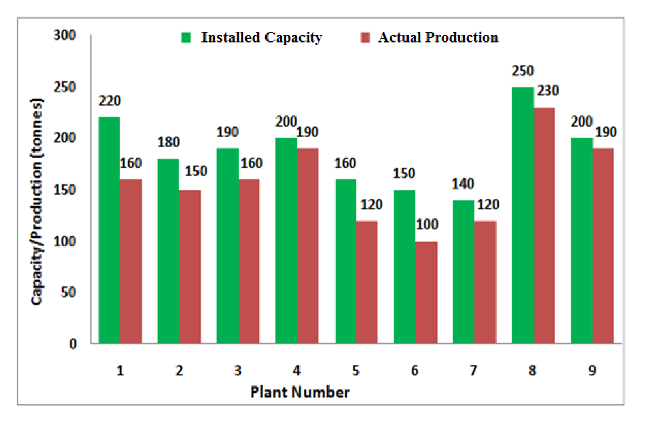
\includegraphics[width=0.5\linewidth]{figs/Figure_1.png}
    \label{fig:enter-label}
\end{figure}

%7
\item A poll of students appearing for masters in engineering indicated that $60\%$ of the students believed that mechanical engineering is a profession unsuitable for women. A research study on women with masters or higher degrees in mechanical engineering found that $99 \%$ of such women were successful in their professions.\\

Which of the following can be logically inferred from the above paragraph? 

    \hfill{[2016-XE]}
\begin{enumerate}
    \item Many students have misconceptions regarding various engineering disciplines.\\
    \item Men with advanced degrees in mechanical engineering believe women are well suited to be mechanical engineers.\\
    \item Mechanical engineering is a profession well suited for women with masters or higher degrees in mechanical engineering.\\
    \item The number of women pursuing higher degrees in mechanical engineering is small.
\end{enumerate}
%8
\item Sourya committee had proposed the establishment of Sourya Institutes of Technology $\brak{\text{SITs}}$ in line with Indian Institutes of Technology $\brak{\text{IITs}}$ to cater to the technological and industrial needs of a developing country.\\

Which of the following can be logically inferred from the above sentence?\\

Based on the proposal, 
\begin{enumerate}[label=(\roman*), leftmargin=3em, labelsep=0.5em, itemindent=1.5em]
    \item In the initial years, SIT students will get degrees from IIT.
    \item SITs will have a distinct national objective.
    \item SIT like institutions can only be established in consultation with IIT.
    \item SITs will serve technological needs of a developing country.
\end{enumerate}
\hfill{[2016-XE]}
\begin{enumerate}
\begin{multicols}{2}
\item $\brak{\text{iii}}$ and $\brak{\text{iv}}$ only
\item $\brak{\text{i}}$ and $\brak{\text{iv}}$ only
\item $\brak{\text{ii}}$ and $\brak{\text{iv}}$ only
\item $\brak{\text{ii}}$ and $\brak{\text{iii}}$ only
\end{multicols}
\end{enumerate}
%9
\item Shaquille O' Neal is a $60\%$ career free throw shooter, meaning that he successfully makes 60 free throws out of $100$ attempts on average. What is the probability that he will successfully make exactly $6$ free throws in $10$ attempts? \hfill{[2016-XE]}\\
\begin{enumerate}
\begin{multicols}{4}
\item $0.2508$
\item $0.2816$
\item $0.2934$
\item $0.6000$
\end{multicols}
\end{enumerate}
%10
\item The numeral in the units position of $211^{870}+146^{127}\times3^{424}$ is \underline{\hspace{1cm}}. \hfill{[2016-XE]}\\
%11
\item A company records heights of all employees. Let $X$ and $Y$ denote the errors in the average height of male and female employees respectively. Assume that $X\sim N\brak{0,4}$ and $Y\sim N\brak{0,9}$ and they are independent. Then the distribution of $Z=\frac{\brak{X+Y}}{2}$ is 

    \hfill{[2016-XE]}
\begin{enumerate}
\begin{multicols}{4}
\item $N\brak{0,6.5}$
\item $N\brak{0,3.25}$
\item $N\brak{0,2}$
\item $N\brak{0,1}$
\end{multicols}
\end{enumerate}
%12
\item The volume of the solid obtained by revolving the curve $y^2=x, 0\leq x \leq 1$ around y-axis is \hfill{[2016-XE]}
\begin{enumerate}
\begin{multicols}{4}
\item $\pi$
\item $2$
\item $\frac{\pi}{2}$
\item $\frac{\pi}{5}$
\end{multicols}
\end{enumerate}
%13
\item Let $y(x)$ be the solution of the initial value problem $\frac{dy}{dx}+2xy=x; y\brak{0}=0$. Find the value of $\lim\limits_{x\to \infty} y(x)$. \hfill{[2016-XE]}
\end{enumerate}

\end{document}
